\chapter{Uitwerking}
\label{ch:uitwerking}
\section{Open Source tools}
Het onderwerp van deze bachelorproef gaat over een vergelijking tussen open-source serverless frameworks voor het draaien van een serverless infrastructuur in house, dit betekend concreet binnen het hele bedrijf. In house duidt op alle infrastructuur waar een organisatie gebruik van maakt, on-premises infrastructuur zoals een eigen datacenter maar ook private cloud behoren hiertoe. Het is van belang om nog even te vermelden dat deze bachelorproef zich focust op het FaaS model en niet op het BaaS model. Nubera biedt momenteel nog geen serverless (FaaS) oplossingen aan klanten, voor hun is dit onderzoek zinvol zodat iedereen binnen Nubera een beeld heeft over wat serverless precies is en hoe dit kan worden opgezet. De requirements waaraan de frameworks moeten voldoen worden opgelijst in volgende sectie. De opzet van deze studie maakt een vergelijking tussen twee open-source frameworks die ik op basis van enkele requirements vergelijk. Een eerste framework waar Nubera interesse in heeft is Fission, dit dient te worden uitgewerkt aan de hand van een Proof-of-Concept. Een tweede framework dat als vergelijking moet dienen mag worden gekozen aan de hand van de requirements die werden vastgelegd.

\section{Requirements analyse}
Hier worden de requirements waaraan de open-source frameworks moeten voldoen opgelijst, zowel functionele als niet-functionele. De requirements worden ook nog eens onderverdeeld in verschillende categorieën volgens prioriteit. De requirements werden gecapteerd in overleg met Nubera.

\subsection{Functionele requirements}
\subsubsection{Must-have}
\begin{itemize}
    \item Kubernetes als onderliggende laag.
    \item Ondersteund serverless functies in Python en GO.
    \item Auto-scalable.
    \item Zo snel mogelijke uitvoeringstijd van functies.
\end{itemize}
\subsubsection{Should-have}
\begin{itemize}
    \item User interface voor makkelijk beheer van functies en API gateways.
    \item Ondersteund serverless functies in Node.js.
    \item YAML format voor templating en definiëring van functies.
\end{itemize}
\subsubsection{Nice-to-have}
\begin{itemize}
    \item Ondersteund serverless functies in nog meer verschillende talen zodat hetzelfde framework kan gebruikt worden bij verschillende klanten.
\end{itemize}
\subsection{Niet-functionele requirements}
\subsubsection{Must-have}
\begin{itemize}
    \item Het moet open-source zijn.
    \item Het framework moet gratis zijn.
    \item Minstens 40 contributors op GitHub.
    \item Minstens 3000 stars op GitHub. (Garantie voor populariteit in de community.)
    \item Gebruiksvriendelijk.
    \item Eenvoudig op te zetten.
\end{itemize}
\subsubsection{Should-have}
\begin{itemize}
    \item Enige maturiteit als garantie voor het functioneren van het framework. (Production ready)
    \item Contributors uit erkende organisaties.
    \item Het project wordt onderhouden, laatste commit is niet ouder dan 2 weken. (Datum van schrijven 13/04/2019)
    \item Goede en duidelijke documentatie.
\end{itemize}
\subsubsection{Nice-to-have}
\begin{itemize}
    \item Slack channel over het project.
\end{itemize}

\section{Long list}
In deze sectie worden alle mogelijke frameworks die in aanmerking komen overeenstemmend met de gecapteerde requirements opgelijst. Per alternatief wordt de website vermeld volgens APA stijl er wordt ook een korte beschrijving gegeven. Na de oplijsting van de verschillende frameworks die in aanmerking komen worden er tabellen opgemaakt waarin terug te vinden is of de frameworks al dan niet aan de requirements voldoen, er is één tabel voor de functionele en één voor de niet-functionele requirements. Op basis van de tabellen worden drie frameworks (inclusief Fission) gekozen die verder worden verwerkt in de short list. De functionele en niet-functionele requirements worden per framework tegen elkaar afgewogen, executietijd van functies, gebruiksvriendelijkheid en eenvoud in installatie zijn niet meetbaar zonder proof-of-concept en zullen maar later in dit onderzoek worden gemeten. Deze requirements worden daarom ook niet in de tabellen opgenomen.

\subsection{Fission}
Fission werd reeds vastgelegd door Nubera en is een Kubernetes native serverless framework voor functies. Het stelt ontwikkelaars in staat functies te schrijven, die een korte levensduur hebben, in verschillende talen. De functies kunnen worden gemapt aan HTTP triggers. \autocite{Fission2019}

\subsection{Kubeless}
\textcite{Kubeless2019} beschrijft zichzelf als een Kubernetes native serverless framework dat ontwikkelaars in staat stelt kleine stukken code of functies op te laden zonder zorg over de onderliggende infrastructuur. Kubeless is de ideale tool voor ieder die op zoek is naar een open-source alternatief voor wat AWS Lambda, Google Cloud Functions en Azure Functions aanbieden.

\subsection{OpenFaaS}
\textcite{OpenFaaS2019} beschrijft zichzelf ook als een framework voor het bouwen van serverless functies met Kubernetes en Docker, het voorziet ook support voor metrics. Tools als Prometheus kunnen makkelijk worden geïmplementeerd voor monitoring.

\subsection{Apache OpenWhisk}
OpenWhisk is een open-source serverless platform dat als respons op events en triggers functies uitvoert. OpenWhisk staat in voor het beheer van de hardware en schaalbaarheid van applicaties met behulp van Docker containers zodat ontwikkelaars zich kunnen focussen op het bouwen van applicaties. \autocite{Apache2019}

\subsection{Fn}
De beschrijving waarmee \textcite{FnProject2019} zichzelf voorstelt luidt als volgt: Het Fn Project is een open-source container-native serverless platform dat overal kan draaien, in elk type van cloud maar ook op locatie. Het is makkelijk in gebruik, ondersteund elke programmeertaal, is uitbreidbaar en performant. 

\subsection{IronFunctions}
\textcite{Iron2018} belooft met hun IronFunctions serverless framework dat taken die veel CPU vragen onmerkbaar in de achtergrond draaien. Het laat ontwikkelaars toe functies te implementeren in applicaties en de focus te leggen op het schrijven van de software. Het voorziet ook snelle en eenvoudige configuratie van de onderliggende infrastructuur en job processing.

\subsection{OpenLambda}
\textcite{OpenLambda2019} is in tegenstelling tot de eerder besproken alternatieven minder ver ontwikkeld. OpenLambda is een framework dat interessant is voor iedereen die wil wil testen en serverless wilt leren kennen. OpenLambda is niet production ready, de eerder besproken tools zijn dit vaak wel al.

\subsection{Nuclio}
Nuclio wordt vaak gebruikt als alternatief voor AWS Lambda. Nuclio is een serverless framework voor functies in real-time en data gedreven applicaties. Nuclio ondersteund ook Kubernetes als platform. \autocite{Nuclio2019}

\subsection{Knative}
\textcite{Pivotal2019} beschrijft Knative als een uitbreiding van Kubernetes die helpt bij het bouwen van moderne, container-gebaseerde applicaties. Knative voorziet een eenvoudige manier voor ontwikkelaars om applicaties bovenop Kubernetes te draaien. Knative is een open-source project in samenwerking met Google.

%bla bla in tabel x en in y worden vergeleken op basis van FR en NFR..
\subsection{Vergelijking}
In tabel \ref{frameworks-fr} worden de verschillende frameworks vergeleken op basis van hun functionele requirements die vooropgesteld  werden.  De tabel duidt de requirements waaraan de frameworks voldoen aan met een ''X'', indien ze niet voldoen volgt er een ''-'' of aangepaste omschrijving. Tabel \ref{frameworks-nfr} geeft een overzicht van de frameworks ten opzichte van de vooropgestelde niet-functionele requirements. In deze tabel geldt hetzelfde: een ''X'' wilt zeggen dat er aan de requirement is voldaan, een ''-'' betekent dat er een requirement niet voldaan is en een aangepaste beschrijving werd gekozen wanneer deze meer zegt dan een ''X'' of ''-''.

\begin{table}[]
    % \centering
    \resizebox{\textwidth}{!}{%
        \begin{tabular}{@{}llccccccccc@{}}
            \toprule
            \multicolumn{2}{l}{} & \textbf{Fission} & \textbf{Kubeless} & \textbf{OpenFaaS} & \textbf{OpenWhisk} & \textbf{Fn} & \textbf{IronFunctions} & \textbf{OpenLambda} & \textbf{Knative} & \textbf{Nuclio} \\ \midrule
            \multirow{3}{*}{\textbf{Must-have}} & Native Kubernetes & X & X & X & X & X & X & X & X & X \\
            & Python/GO support & X & X & X & X & X & X & Enkel Python & X & X \\
            & Auto-scalable & X & X & X & X & X & - & - & X & X \\
            \hline
            \multirow{3}{*}{\textbf{Should-have}} & User-interface & X & X & X & - & X & X & - & - & X \\
            & Node.js support & X & X & X & X & X & X & - & X & X \\
            & YAML templating & X & X & X & X & X & - & - & X & X \\
            \hline
            \textbf{Nice-to-have} & Support voor meer talen & X & X & X & X & X & X & - & X & X \\ \bottomrule
        \end{tabular}%
    }
    \caption{Vergelijking serverless frameworks op basis van functionele requirements}
    \label{frameworks-fr}
\end{table}


\begin{table}[]
    \resizebox{\textwidth}{!}{%
        \begin{tabular}{@{}llccccccccc@{}}
            \toprule
            &  & \textbf{Fission} & \textbf{Kubeless} & \textbf{OpenFaaS} & \textbf{OpenWhisk} & \textbf{Fn} & \textbf{IronFunctions} & \textbf{OpenLambda} & \textbf{Knative} & \textbf{Nuclio} \\ \midrule
            \multirow{4}{*}{\textbf{Must-have}} & Open-source & X & X & X & X & X & X & X & X & X \\
            & Gratis & X & X & X & X & X & X & X & X & X \\
            & > 40 contributors & 76 & 77 & 99 & 151 & 77 & 32 & 17 & 115 & 36 \\
            & > 3K GitHub stars & 4.2K & 4.5K & 13.8K & 3.9K & 3.9K & 2.5K & 593 & 1.6K & 2.6K \\
            \hline
            \multirow{4}{*}{\textbf{Should-have}} & Maturiteit (Production ready) & X & X & X & X & X & - & - & X & X \\
            & Mede ontwikkeld door erkende organisaties & Platform9 & Bitnami & VMWare & IBM & Oracle & iron.io & - & Google & - \\
            & Laatste commit (datum schrijven 13/04/2019) & 09/04/2019 & 09/04/2019 & 13/04/2019 & 11/04/2019 & 10/04/2019 & 20/08/2018 & 14/01/2019 & 13/03/2019 & 01/04/2019 \\
            & Goede/duidelijke documentatie & X & X & X & X & - & - & - & X & X \\
            \hline
            \textbf{Nice-to-have} & Slack channel over het project & X & X & X & X & X & - & - & X & X \\ \bottomrule
        \end{tabular}%
    }
    \caption{Vergelijking serverless frameworks op basis van niet-functionele requirements}
    \label{frameworks-nfr}
\end{table}

\subsubsection{Resultatenverwerking}
Eerst worden de functionele requirements behandelt. Op basis van tabel \ref{frameworks-fr} is onmiddellijk zichtbaar dat enkele frameworks minder interessant zijn dan anderen. IronFunctions en OpenLambda voldoen niet aan de must-have requirements en worden dus niet verder behandelt. OpenWhisk en Knative worden niet geleverd met een user interface en voldoen zo beiden niet aan de should-have functionele requirements. Alle overige kandidaten voldoen aan de nice-to-have requirements, namelijk ondersteuning voor meerdere programmeertalen.
\\\\
Vervolgens worden de niet-functionele requirements bekeken. De tabel weergeeft dat alle frameworks open-source en gratis zijn, deze requirements worden dus voor alle frameworks voldaan. De volgende requirements die in acht worden genomen zijn het aantal contributors eveneens als het aantal ''stars'' op GitHub. Een hoger aantal contributors wijst vaak op meer kennis, meer review van code en enige zekerheid in vergelijking met een laag aantal contributors. De GitHub stars worden als factor gekozen om te meten hoe populair een framework is. De metingen werden gedaan op 13 april 2019 en kunnen tegen de tijd van lezen reeds gewijzigd zijn. Als norm werd vooropgesteld dat een project minstens veertig contributors moet hebben alsook een minimum van drieduizend stars. IronFunctions, OpenLambda en Nuclio voldoen niet aan het opgelegde aantal contributors. Knative, OpenLambda, Nuclio en IronFunctions behalen ook niet het minimum van drieduizend stars. Daarnaast worden ook de should-have requirements bekeken. Alle kandidaat frameworks voldoen aan maturiteit en zijn ''production ready''. Elk framework behalve Nuclio en OpenLambda wordt mede ontwikkeld door erkende organisaties, de bedrijven die werden opgelijst worden ook wel de ''backers'' van het project genoemd. Omdat Nuclio en OpenLambda geen erkende organisatie achter zich hebben worden deze kandidaten niet meer in overweging genomen. De datum van de laatste commit is ook een belangrijk gegeven om te beslissen of het project overlevingskans heeft en up-to-date blijft. Bij Knative dateert de laatste commit van een maand geleden wat erg lang is voor een open-source project, ook deze optie wordt geschrapt. De overige kandidaten beschikken allemaal over een duidelijke documentatiewebsite, videobronnen en Slack channels om over het project te praten. Tabel \ref{frameworks-samenvattingl} weergeeft een samenvatting van de frameworks en het aantal requirements waaraan ze voldoen, ze worden gerangschikt volgens de graad dat ze in aanmerking komen, van boven naar beneden. In de tabel wordt telkens voor de verschillende categorieën van requirements een optelling gemaakt waaraan een framework voldoet. Uit de tabel is af te leiden dat OpenFaaS, Kubeless en Fission een maximumscore behalen en dus ook het meest interessant zijn voor verder onderzoek. In sectie \ref{sec:short-list} worden deze drie frameworks verder in detail besproken. Nubera gaf aan dat zij interesse hebben in Fission, dit framework zal worden opgezet in een proof-of-concept, daarnaast wordt ook nog een alternatief, OpenFaaS of Kubeless opgezet als vergelijking. Aan de hand van de uitwerking moet blijken of Fission een goede keuze is of dat een ander alternatief misschien nog meer mogelijkheden biedt.
\\
\begin{table}[]
    \centering
    \resizebox{\textwidth}{!}{%
        \begin{tabular}{@{}llccccccccc@{}}
            \toprule
            &  & \multicolumn{3}{c}{\textbf{Functionele requirements}} & \textbf{} & \multicolumn{3}{c}{\textbf{Niet-functionele requirements}} & \textbf{} & \textbf{Totaal} \\ \midrule
            &  & \textbf{M-H} & \textbf{S-H} & \textbf{N-T-H} & \textbf{} & \textbf{M-H} & \textbf{S-H} & \textbf{N-T-H} & \textbf{} & \textbf{/16} \\
            \textbf{1.} & \textbf{OpenFaaS} & 3 & 3 & 1 &  & 4 & 4 & 1 &  & 16 \\
            \textbf{2.} & \textbf{Kubeless} & 3 & 3 & 1 &  & 4 & 4 & 1 &  & 16 \\
            \textbf{3.} & \textbf{Fission} & 3 & 3 & 1 &  & 4 & 4 & 1 &  & 16 \\
            \textbf{4.} & \textbf{OpenWhisk} & 3 & 2 & 1 &  & 4 & 4 & 1 &  & 15 \\
            \textbf{5.} & \textbf{Fn} & 3 & 3 & 1 &  & 4 & 3 & 1 &  & 15 \\
            \textbf{6.} & \textbf{Knative} & 3 & 2 & 1 &  & 3 & 4 & 1 &  & 14 \\
            \textbf{7.} & \textbf{Nuclio} & 3 & 3 & 1 &  & 2 & 3 & 1 &  & 13 \\
            \textbf{8.} & \textbf{IronFunctions} & 2 & 2 & 1 &  & 2 & 1 & 0 &  & 8 \\
            \textbf{9.} & \textbf{OpenLambda} & 1 & 0 & 0 &  & 2 & 0 & 0 &  & 3 \\
            &  & \multicolumn{1}{l}{} & \multicolumn{1}{l}{} & \multicolumn{1}{l}{} & \multicolumn{1}{l}{} & \multicolumn{1}{l}{} & \multicolumn{1}{l}{} & \multicolumn{1}{l}{} & \multicolumn{1}{l}{} & \multicolumn{1}{l}{} \\
            &  & \multicolumn{1}{l}{} & \multicolumn{1}{l}{} & \multicolumn{1}{l}{} & \multicolumn{1}{l}{} & \multicolumn{1}{l}{} & \multicolumn{1}{l}{} & \multicolumn{1}{l}{} & \multicolumn{1}{l}{} & \multicolumn{1}{l}{} \\ \bottomrule
        \end{tabular}%
    }
    \caption{Frameworks opgelijst in graad waarin ze in aanmerking komen. De top drie van meest interessante frameworks voor dit onderzoek zijn OpenFaaS, Kubeless en Fission. Door Nubera werd zelf aangegeven dat ze interesse hebben in Fission. (M-H: Must-have, S-H: Should-have, N-T-H: Nice to have.) }
    \label{frameworks-samenvattingl}
\end{table}

\section{Short List}
\label{sec:short-list}

In deze sectie wordt op basis van voorgaande long list, zoals eerder al aangehaald, drie frameworks die aan de meeste/alle requirements voldoen verder behandelt. Nubera wilt zeker verdere informatie en proof-of-concept over Fission, daarnaast willen ze ook een evenwaardig alternatief zodat op basis van dit onderzoek een keuze kan gemaakt worden. De verdere uitwerking tracht ook de requirments die nog niet werden gemeten te behandelen. De functionele requirement: ''Zo snel mogelijke uitvoeringstijd van functies.'' en de niet-functionele requirements: ''Gebruiksvriendelijk'' en ''Eenvoudig op te zetten'' worden in de proof-of-concept verder onderzocht. Op basis van de shortlist kiezen wordt het meest veelbelovende alternatief voor Fission gekozen, de proof-of-concept bestaat dan uit een vergelijking tussen dit gekozen framework en Fission.


\subsection{OpenFaaS}
\textcite{OpenFaaS2019} is een open-source Function as a Service (serverless) project dat werd opgestart door Alex Ellis. Alex is lid van het VMWare Open Source Technology Center (OSTC), VMWare is eveneens ''backer'' van dit project, ze ondersteunen in de ontwikkeling van OpenFaaS. Het project telt 13.8K GitHub stars, 99 contributors en is daarmee momenteel het grootste en populairste open-source Function as a Service framework. OpenFaaS wordt al gebruikt bij verschillende grote organisaties zoals: VMWare, BT (British Telecom), Citrix, Contiamo, University of Washington, ... 
\\
De aspecten waarmee OpenFaaS uitpakt om zich te onderscheiden van anderen zijn:
\begin{itemize}
    \item Makkelijke installatie en eenvoud in gebruik door de beschikbare UI.
    \item Portable: draait op bestaande hardware of in de public/private cloud maar ook op Kubernetes of Docker Swarm.
    \item Functies in eender welke taal voor Linux of Windows.
    \item Auto-scalable wanneer de vraag verhoogt.
    \item YAML format voor templating en definiëren van functies.
\end{itemize}
\subsubsection{Conceptueel ontwerp}
OpenFaaS kan worden opgedeeld in verschillende onderdelen met elk hun eigen verantwoordelijkheden.
\begin{figure}
    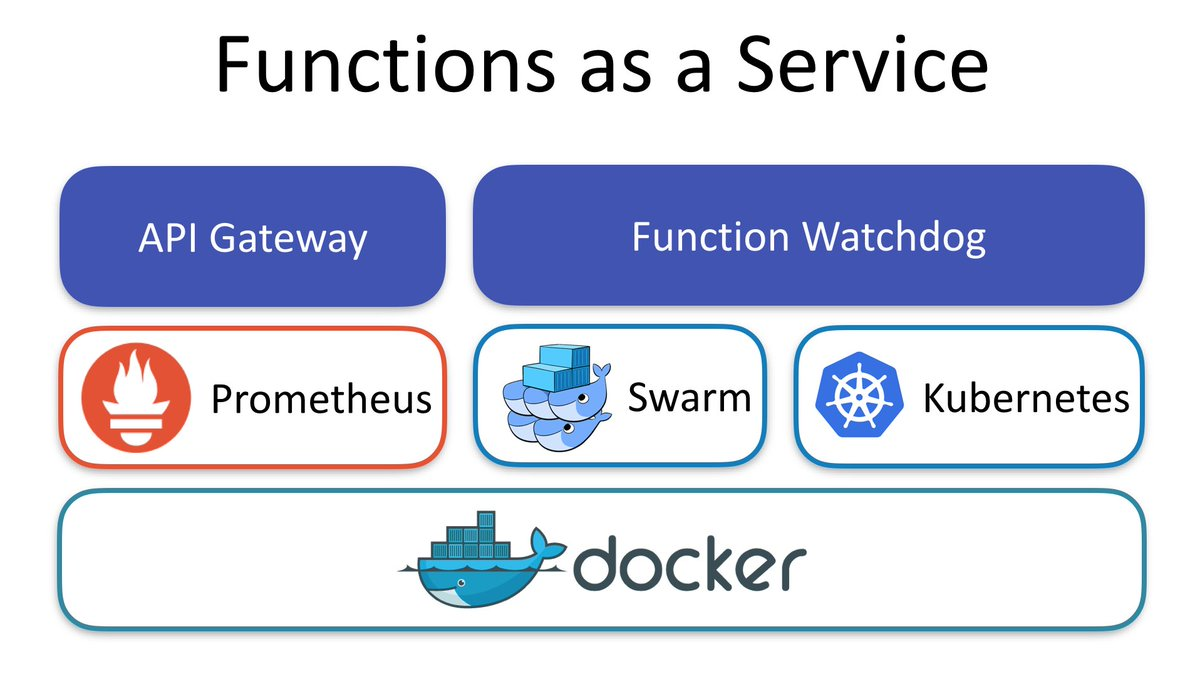
\includegraphics[width=1\textwidth]{img/open-faas.jpg}
    \caption{De figuur weergeeft een conceptuele voorstelling van de componenten van OpenFaaS. \autocite{Ellis2019}}
    \label{fig:open-faas-conceptueel}  
\end{figure}

\begin{description}[style=unboxed, labelwidth=\linewidth, listparindent =0pt]
    \item[Docker laag]
    In figuur \ref{fig:open-faas-conceptueel} is de onderste laag een volledige Docker laag, dit weergeeft dat alle functies die geschreven worden worden uitgevoerd in Docker containers, deze containers bevatten alle dependencies nodig voor de code om uit te voeren.
    \newline
    
    \item[Swarm/Kubernetes]
    Bovenop de Docker laag in figuur \ref{fig:open-faas-conceptueel} is er een Swarm of Kubernetes component terug te vinden. Deze laag is de zogenoemde ''orchestrator'', deze staat in voor het management, configuratie en de coördinatie van de Docker containers.
    \newline
    
    \item[Prometheus]
    OpenFaaS maakt gebruik van Prometheus, een tool voor het verzamelen van metrics.
    \newline
    
    \item[Function Watchdog]
    In figuur \ref{fig:open-faas-conceptueel} staat de Function Watchdog bovenop de reeds opgesomde componenten. Function Watchdog zorgt ervoor dat een Docker image kan worden omgevormd in een serverless functie, dit door het toevoegen van een kleine HTTP server. Daarnaast is de Function Watchdog eveneens het ingangspunt dat HTTP requests toelaat om geforward te worden naar het bestemmingsproces via HTTP of STDIN. Het responsbericht wordt teruggestuurd naar STDOUT of HTTP van de applicatie. \autocite{Ellis2019}
    \newline
    
    \item[API Gateway/UI Portal]
    De API Gateway in figuur \ref{fig:open-faas-conceptueel} verzorgt een route naar de geschreven functies en verzameld metrics aan de hand van Prometheus. De API Gateways zorgt eveneens voor schaalbaarheid van Functies door de vraag op te halen via de replica count in Docker Swarm of de Kubernetes API. Bij installatie van OpenFaaS wordt er ook een UI meegeleverd, deze laat gebruikers toe functies op te vragen en toe te voegen via deze interface. \autocite{Ellis2019} 
    \newline
    
    \item[CLI]
    Elk proces binnen een container of de container op zich kan een serverless functie zijn. OpenFaaS voorziet FaaS CLI om snel functies te deployen. Nieuwe functies kunnen worden gemaakt aan de hand van templates maar ook via een Dockerfile. \autocite{Ellis2019}  
\end{description}

\subsection{Kubeless}
\textcite{Kubeless2019} is een Kubernetes native serverless framework. Het is ontwikkeld om bovenop een Kubernetes cluster te worden geïnstalleerd. De eerste commit aan het Kubeless project dateert van 16 november 2016 en werd gemaakt door iemand met de naam ''ngtuna'' op GitHub. Kubeless is goed voor 5K GitHub stars en heeft telt momenteel 77 contributors. Bitnami is de ondersteunende organisatie achter Kubeless. Organisaties die reeds Kubeless implementeren zijn moeilijk terug te vinden in tegenstelling tot OpenFaaS gebruikers, dit wijst mogelijks op een grotere maturiteit van OpenFaaS ten opzichte van Kubeless. 
\\
Kubeless zegt zelf het beste alternatief te zijn voor de serverless oplossingen die de grote spelers vandaag reeds aanbieden. De aspecten eigen aan Kubeless zijn:
\begin{itemize}
    \item Ondersteuning voor Python, Node.js Ruby, Golang, PHP, .NET, Ballerina en nog meer custom runtimes.
    \item CLI gelijkaardig aan die van AWS Lambda.
    \item Event triggers en HTTP events.
    \item Plugin voor gebruik van het Serverless framework. \autocite{Serverless2018}
    \item Standaard monitoring van functies die worden aangeroepen en latency aan de hand van Prometheus.
\end{itemize}

\subsubsection{Architectuur}
Kubeless is gebouwd rond drie concepten die hieronder verder in detail worden toegelicht.
\begin{description}[style=unboxed, labelwidth=\linewidth, listparindent =0pt]
    \item[Functies]
    Een functie is een representatie van de code die moet worden uitgevoerd. Naast code bevat een functie ook metadata over de runtime dependencies alsook build instructies. De levensduur van een functie staat niet vast, de functie wordt ook enkel uitgevoerd wanneer een trigger deze activeert. \autocite{KnightXun2018}
    \newline
    
    \item[Triggers]
    Een trigger reageert op binnenkomende  events, aan de triggers worden functies gekoppeld. Wanneer er een event voorkomt zal Kubeless ervoor zorgen dat de corresponderende functie wordt aangeroepen, het event zorgt ervoor dat de trigger op de hoogte wordt gebracht en die roept bijgevolg de juiste functie aan. Een trigger kan bij een of meerdere functie horen en staan ook los van deze functies. Triggers worden apart onderhouden en geconfigureerd los van de functies. \autocite{KnightXun2018}
    \newline
    
    \item[Runtime]
    Een runtime staat in voor de taal en de taal-specifieke omgeving waarin functies worden uitgevoerd. Elke specifieke taal heeft een andere runtime, zo heeft Java een andere runtime dan Python nodig voor de uitvoering van code. \autocite{KnightXun2018}
    \newline
\end{description}


\subsection{Fission}
Fission is een framework voor serverless functies op Kubernetes dat werd aangegeven door Nubera zelf, na verder onderzoek bleek dit ook te voldoen aan alle opgestelde requirements. Fission bestaat sinds augustus 2016 en wordt ontwikkeld door medewerkers van Platform9. Momenteel Heeft Fission 4K stars op GitHub en 76 contributors. Gebruikers die Fission reeds in hun organisatie implementeren zijn eveneens een stuk moeilijker te vinden in vergelijking met OpenFaaS.
\\
De  belangrijkste aspecten van Fission zijn:
\begin{itemize}
    \item Native Kubernetes: Fission draait op elke locatie op Kubernetes.
    \item Snelle cold-start: functies hebben een korte cold-start latency, lager dan ~100ms.
    \item Functie samenstelling: Fission Workflows zorgt ervoor dat ontwikkelaars niet moeten bezig zijn met networking, bericht wachtrijen of andere onderdelen die serverless functies complex maken.
    \item Administratie en operationele eenvoud: logs worden onmiddellijk via de CLI weergegeven daarnaast is er ook integratie met Prometheus voor het evalueren van metrics aan de hand van een duidelijk dashboard.
    \item Istio integratie: Fission integreert met Istio, een platform dat instaat voor management en beveiliging van microservices. Via dashboards kunnen gebruikers ook informatie ophalen over de latency van functies die worden aangeroepen.
    \item Declaratie van functies moet maar éénmaal door de ontwikkelaar worden gedaan, vervolgens kan de functie overal worden gedeployed.
    \item Ondersteuning voor meerdere programmeertalen: Python, Node.js, GO, C#, PHP daarnaast kunnen ook eigen containers worden gebouwd indien dit nodig is. 
    \item Auto-scaling van functies. 
\end{itemize}

\subsubsection{Architectuur}


\subsection{Verschillen en overweging}